\documentclass[../main.tex]{subfiles}

\begin{document}
\begin{questions}

\question A metal sphere with radius $R_1$ has charge $Q$. A second metal sphere with radius $R_2$ has zero charge. Now connect the spheres together using a fine conducting wire. Assume that the spheres are separated by a distance $R$ which is large enough that the charge distribution on each ball remains uniform. Derive an expression for the final charge on the sphere with
radius $R_1$.
\begin{solution}
	\begin{center}
		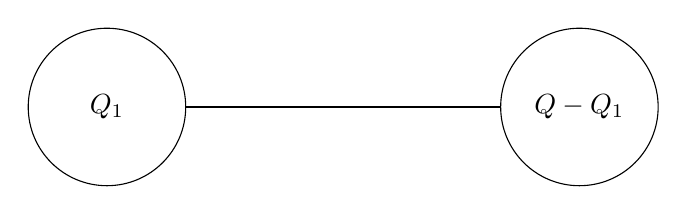
\begin{tikzpicture}
			\draw (-3,0) circle (1) node {$Q_1$};

			\draw (3,0) circle (1) node {$Q-Q_1$};

			\draw (-2,0) -- (2,0);
		\end{tikzpicture}
	\end{center}

	We need to equate the potentials at each end of the wire, because that is when the whole conductor system will become an equipotential
	% \begin{align}
	% 	V_\text{left end} &= V_\text{right end}\\
	% 	\frac{Q_1}{R_1} + \frac{Q-Q_1}{R} &= \frac{Q-Q_1}{R_2} + \frac{Q_1}{R}\\
	% 	\implies Q_1 &= \frac{(R-R_2)R_1}{RR_1+RR_2-2R_1R_2}
	% 	\intertext{$R \gg R_1,R_2$}
	% 	\implies Q_1 &= Q\frac{\left(1-\frac{R_2}{R}\right)}{1-2\frac{R_2}{R\left(1+\frac{R_2}{R_1}\right)}\left(1+\frac{R_2}{R_1}\right)}

	% \end{align}

	\begin{align}
		V_\text{left end} &= V_\text{right end}\\
		\frac{Q_1}{R_1} + \frac{Q-Q_1}{R} &= \frac{Q-Q_1}{R_2} + \frac{Q_1}{R}\\
		\implies Q_1 &= \frac{(R-R_2)R_1}{RR_1+RR_2-2R_1R_2}
		\intertext{$R \gg R_1,R_2$}
		\implies Q_1 &= Q\frac{\left(1-\frac{R_2}{R}\right)}{\left(1-2\frac{R_2}{R\left(1+\frac{R_2}{R_1}\right)}\right)\left(1+\frac{R_2}{R_1}\right)}\\
		&\approx Q\frac{R_1}{R_1+R_2}\left(1-\frac{R_2}{R}\right)\left(1+2\frac{R_2}{R\left(1+\frac{R_2}{R_1}\right)}\right)\\
		&\approx Q\frac{R_1}{R_1+R_2}\left(1+\frac{R_2(R_1-R_2)}{R(R_1+R_2)}\right)
	\end{align}
\end{solution}

\question
\begin{parts}
	\part Show that the capacitance, $C$, of a conducting sphere of radius $a$ is given by $C$ = $4\pi\epsilon_0a$
	\begin{solution}
		Assume a conducting sphere of radius a carrying a total charge Q, which will be distributed uniformly. Potential on surface of the sphere is 
		\[\frac{Q}{4\pi\epsilon_0a}\] \\
		Since our reference for potential measurement is with respect to infinity, potential at infinity is 0
		Hence, Capacitance is 
		\begin{equation}C = \frac{Q}{V} = 4\pi\epsilon_0a \end{equation}
	\end{solution}

	\part Two isolated conducting spheres, both of radius $a$, initially carry charges of $q_1$ and $q_2$ and are held far apart. The spheres are connected together by a conducting wire until equilibrium is reached, whereupon the wire is removed. Show that the total electrostatic energy stored in the spheres decreases by an amount $U$ , given by \[\Delta U= \frac{1}{16\pi\epsilon_0a}(q_1-q_2)^2\]
    What happens to this energy?
	\begin{solution}
		Initial Charges on the spheres are $q_1$ and $q_2$. When the spheres are connected by the wire, they become equipotential. Assume the final charges are $q_1'$ and $q_2'$
		\begin{align}
			\notag q_1+q_2 &= q_1'+q_2' \\
			\notag\frac{q_1'}{4\pi\epsilon_0a} &= \frac{q_2'}{4\pi\epsilon_0a} \\
			\notag\implies q_1'=q_2'&=\frac{q_1+q_2}{2}
			\intertext{Initial Energy is}
			\notag E_1 &= \frac{q_1^2+q_2^2}{2C}
			\intertext{Final Energy is}
			\notag E_2 &= \frac{q_1'^2+q_2'^2}{2C}
			\intertext{Substituting }
			\Delta U &= \frac{1}{16\pi\epsilon_0a}(q_1-q_2)^2
		\end{align}
		As the charges move from one sphere to another under the influence of an electric field(higher to lower potential), they gain kinetic energy. When the reach the second sphere, this energy gets dissipated as heat. In other words, this energy gets dissipated due to resistive heating of the wire
	\end{solution}
\end{parts}

\question A metal sphere of radius $R$ carries a total charge $Q$. What is the force of repulsion between the "northern" hemisphere and the "southern" hemisphere?
\label{q:hemi}
\begin{solution}
	Since the sphere is made of metal(conductor), all the charge will be uniformly distributed on the surface(with $\sigma=\frac{Q}{4\pi R^2}$). Let $\mathcal S$ represent the surface of the "northern" hemisphere. 
    Electrostatic Pressure $P=\frac{\sigma^2}{2\epsilon_0}=\frac{Q^2}{32\pi^2\epsilon_0R^4}$
    \begin{align} 
        F = \oiint_{\mathcal S} P(r)\,d\Vec{A}
        \intertext{By symmetry, we know that force along $z$-axis only will survive. Hence we take the component of each elemental contribution to force along with $z$-axis}
        F &= \oiint_{\mathcal S}\frac{Q^2}{32\pi^2\epsilon_0R^4}\cos\theta\,d\Vec{A} \\
        &= \frac{Q^2}{32\pi^2\epsilon_0R^4}\int_{\phi=0}^{2\pi}\int_{\theta=0}^{\frac{\pi}{2}}R^2\cos\theta \sin\theta \,d\theta \,d\phi \\
        \implies F &= \frac{Q^2}{32\pi\epsilon_0R^2}
    \end{align}
\end{solution}

\question  A solid spherical conductor encloses 3 cavities, a cross-section of which are as shown in the figure. A net charge $+q$ resides on the outer surface of the conductor. Cavities A and C contain point charges $+q$ and $-q$, respectively. What are the net charges on the surfaces of the cavities?
\begin{center}
	\begin{tikzpicture}
		\draw[pattern={Lines[angle=-45,distance={5pt}, line width=1pt]}, pattern color=white,even odd rule] (0,0) circle (2) (0,1) node{$B$} \irregularcircle{0.5cm}{0.1cm} (-1,0) circle (0.7) node {\textbullet} node[xshift=0cm,yshift=-0.3cm]{$+q$} node[xshift=0cm,yshift=0.3cm]{$A$} (1,0) ellipse (0.45cm and 0.85cm) node {\textbullet} node[xshift=0cm,yshift=-0.3cm]{$-q$} node[xshift=0cm,yshift=0.3cm]{$C$};

		\node at ({-2*cos(45)},{2*sin(45)}) [anchor=south east]{$+q$};
	\end{tikzpicture}
\end{center}

\begin{solution}
	Consider a Gaussian surface just outside the cavity A inside the interior of the bulk of the conductor. Since electric field is 0 everywhere inside the bulk of a conductor, flux through the Gaussian surface is 0. By Gauss' Law, the net charge inside the Gaussian surface is 0. Hence,\[Q_{inside\ cavity}+Q_{on\  surface}=0\]
    Hence charge on surface of cavity A = $-q$ \\
    Similarly, charge on surface of cavity C = $+q$
\end{solution}

\question A metal sphere of radius $R$, carrying charge $q$, is surrounded by a thick concentric metal shell (inner radius $a$, outer radius $b$). The shell carries no net charge.
\begin{parts}
	\part Find the surface charge density $\sigma$ at $R$, at $a$, and at $b$.

	\begin{solution}
		$\sigma_R = \frac{q}{4\pi R^2}$, as any leftover charge on conductor will distribute itself uniformly on the surface\\
		This $+q$ in the cavity of the shell induces a total charge of $-q$ on the inner surface of shell. Hence $\sigma_a=\frac{-q}{4\pi a^2}$\\
		The leftover charge on shell distributes itself uniformly on the outer surface. Hence $\sigma_b = \frac{q}{4\pi b^2}$
	\end{solution}

	\part Find the potential at the center, using infinity as the reference point.
	\begin{solution}
		$V(b) = \frac{q}{4\pi\epsilon_0b}$ (The interior of shell is shielded)\\
		$V(a) = V(b)$\\
		$V(R) = V(a) + \frac{q}{4\pi\epsilon_0}\left(\frac{1}{R}-\frac{1}{a}\right)$\\
		$V(a)=V(R) = \frac{q}{4\pi\epsilon_0}\left(\frac{1}{b}-\frac{1}{a}+\frac{1}{R}\right)$
	\end{solution}

	\part Now the outer surface is touched to a grounding wire, which drains off charge and lowers its potential to zero (same as at infinity). How do your answers to (a) and (b) change?
	\begin{solution}
		The only difference is there will be no leftover charge $+q$ on the outer surface of shell. So $\sigma_b=0$\\
		Also, $V(a)=V(b)=0$\\
		So $V(0)=\frac{q}{4\pi\epsilon_0}\left(\frac{1}{R}-\frac{1}{a}\right)$
	\end{solution}
\end{parts}

\question A point charge $q$ of mass $m$ is released from rest at a distance $d$ from an infinite grounded conducting plane. How long will it take for the charge to hit the plane?
\begin{solution}
	We will first find the velocity of the charge after falls to a distance of $x$ from the plane, by energy conservation
	\begin{align*}
		\frac{1}{2}mv^2 &= \frac{q^2}{16\pi\epsilon_0} \left( \frac{1}{x} - \frac{1}{d} \right) \\
		\implies v &= \sqrt{\frac{q^2}{8\pi\epsilon_0m} \left( \frac{1}{x} - \frac{1}{d} \right)} \\
		\implies T &= \sqrt{\frac{8\pi\epsilon_0m}{q^2}}\int^{x=0}_{x=d} \left( \frac{1}{x} - \frac{1}{d} \right)^{-\frac{1}{2}} \\
		&= \frac{\pi d}{q}(2\pi\epsilon_0md)^{\frac{1}{2}}
	\end{align*}
\end{solution}


\question Two infinite parallel grounded conducting plates are held a distance $a$ apart. A point charge $q$ is placed between them, at a distance $x$ from one plate. Find the force on $q$. Check that your answer is correct for the special cases $a \to \infty$ and $x = \frac{a}{2}$.
\begin{solution}
	\begin{center}
		\includegraphics[width=\textwidth]{assets/grif3-39.png}
	\end{center}
	The image configuration is shown in the figure, the positive image charges cancel in pairs. The net force of the negative image charges is:
	\begin{align}
		F &= \frac{1}{4\pi\epsilon_0}q^2\Biggr\{ \frac{1}{[2(a-x)]^2} + \frac{1}{[2a + 2(a-x)]^2} + \frac{1}{[4a + 2(a-x)]^2} + \hdots\\
		& -\frac{1}{(2x)^2} - \frac{1}{(2a + 2x)^2} - \frac{1}{(4a + 2x)^2} - \hdots \Biggr\} \\
		&= -\frac{q^2}{16\pi\epsilon_0}\left\{ \sum^\infty_{n=0} \frac{1}{(na+x)^2} - \sum^\infty_{n=1}\frac{1}{(na-x)^2} \right\} \\
		&= -\frac{q^2}{16\pi\epsilon_0}\left\{ \frac{1}{x^2} - 4ax\sum^{\infty}_{n=1} \frac{n}{(n^2a^2-x^2)^2} \right\}
	\end{align}
	Now when $a\to\infty$, the sum term tends to $0$, and we are left with
	\begin{equation}
		F = \frac{q^2}{4\pi\epsilon_0}\frac{1}{(2x)^2}
	\end{equation}
	which is the same force as the case for a single plane. \\
	If $x=\frac{a}{2}$ then we expect no force, and:
	\begin{equation}
		F = \frac{q^2}{16\pi\epsilon_0}\left\{ \frac{4}{a^2} - \frac{2}{a^2}\sum^\infty_{n=1}\frac{n}{\left(n^2-\frac{1}{4}\right)^2} \right\} = 0
	\end{equation}
\end{solution}

\question A conducting sphere (or a shell) of radius $R$ has a charge $Q$.
\begin{parts}
	\part Find the force of repulsion between the two hemispheres
	\begin{solution}
		Already calculated in \ref{q:hemi}
	\end{solution}

	\part Now suppose one has a solid sphere of radius $R$ with charge $Q$ distributed uniformly over its volume.
	\begin{solution}
		Let $\mathcal V$ represent the volume of the sphere.
		\begin{align}
			\Vec{F} &= \iiint_{\mathcal V}\rho\vec{E}(r)d\tau \\
			&= \iiint_{\mathcal V}\frac{3Q}{4\pi\epsilon_0R^3}\frac{Qr\hat{r}}{4\pi\epsilon_0R^3}d\tau
			\intertext{Since we know field is in $z$-direction by symmetry}
			&= \iiint_{\mathcal V}\frac{3Q}{4\pi R^3}\frac{Qr}{4\pi\epsilon_0R^3}\cos\theta d\tau \\
			&= \frac{3Q^2}{16\pi^2\epsilon_0R^6}\int_{r=0}^R\int_{\phi=0}^{2\pi}\int_{\theta=0}^{\frac{\pi}{2}}r^3\cos\theta \sin\theta \,dr \,d\theta\, d\phi \\
			\implies F &= \frac{3Q^2}{64\pi\epsilon_0R^2}
		\end{align}
	\end{solution}

	\part  Which case (a) vs (b) has the larger force of repulsion?
	\begin{solution}
		Clearly, the force of repulsion is greater in (b) than (a) as in the case of the conductor, the charges redistribute to minimise repulsion.
	\end{solution}
\end{parts}

\question 
\begin{parts}
	\part Find the average potential over a spherical surface of radius $R$ due to a point charge $q$ located inside. Show that, in general,
	\begin{equation*}
		V_\text{ave} = V_\text{center} + \frac{Q_{enc}}{4\pi\epsilon_0 R}
	\end{equation*}
	where $V_{center}$ is the potential at the center due to all the external charges and $Q_{enc}$ is the total enclosed charge.
	\begin{solution}
		The average value of $V$ at a point $r$ over a spherical surface of radius $R$ is given as (assuming $\mathcal{S}$ represents the sphere surface)
		\begin{equation}
		V_\text{ave}(r)=\frac{1}{4\pi R^2}\oiint_{\mathcal{S}} V\,dS
		\end{equation}
		In this case since the point charge is located inside so we can break $V_\text{ave}=V_\text{int}+V_\text{ext}$ where $V_\text{int}$ is the average due to the internally located charges and $V_\text{ext}$ is the due to the externally located charges.\\
		The potential $V_\text{int}$ due to the point charge $q$ located inside the sphere at $\vec{r'}=(0,0,z)$ can be calculated as follows 
		\begin{align}
		V_\text{int} &= \frac{1}{4\pi R^2}\oiint_{\mathcal{S}}\left(\frac{1}{4\pi\epsilon_0}\frac{q}{|\vec{r}-\vec{r'}|}\right) \,dS\\
		&=\frac{q}{16\pi^2\epsilon_0 R^2}\int_{\theta=0}^{\pi}\int_{\phi=0}^{2\pi} \frac{1}{\sqrt{R^2+z^2-2zR\cos\theta}}R^2\sin\theta\,d\theta\,d\phi\\
		&= \frac{q}{8\pi\epsilon_0}\int_{\theta=0}^{\pi} \frac{\sin\theta}{\sqrt{R^2+z^2-2zR\cos\theta}}\,d\theta\\
		&=\frac{q}{4\pi\epsilon_0R}
		\end{align}
		Thus from superposition principle, $V_\text{int}=\frac{Q_\text{enc}}{4\pi\epsilon_0R}$

		For $V_\text{ext}$, the potential is same as given at the center of the sphere $V_\text{center}$.

		So finally, we have 
		$$
		V_\text{ave} = V_\text{center} + \frac{Q_{enc}}{4\pi\epsilon_0 R}
		$$
	\end{solution}

	\part Find the general solution to Laplace's equation in spherical coordinates for the
	case where $V$ depends only on $r$. Do the same for cylindrical coordinates assuming $V$ depends only on $s$.
	\begin{solution}
		In case of the spherical coordinates we will have 
		$$
		\nabla^2 V= \frac{1}{r^2}\frac{d}{dr}\left(r^2\frac{dV}{dr}\right)=0
		$$
		for which the solution will be 
		$$
		V = \frac{-c}{r}+k
		$$
		where $c,k$ is some constant.

		In case of the cylindrical coordinates we will have 
		$$
		\nabla^2 V= \frac{1}{s}\frac{d}{ds}\left(s\frac{dV}{ds}\right)=0
		$$
		and the solution for the above case is 
		$$
		V = c\ln s+k
		$$
		where $c,k$ is some constant.
	\end{solution}
\end{parts}

\question A point charge $+q$ is placed at a distance $d$ from the centre of a conducting sphere of radius $R$ ($d > R$). Show that if the sphere is grounded, the ratio of the charge on the part of the sphere visible from $+q$ to that on the rest is $\sqrt{\frac{d+R}{d-R}}$.
\begin{solution}
	\begin{center}
		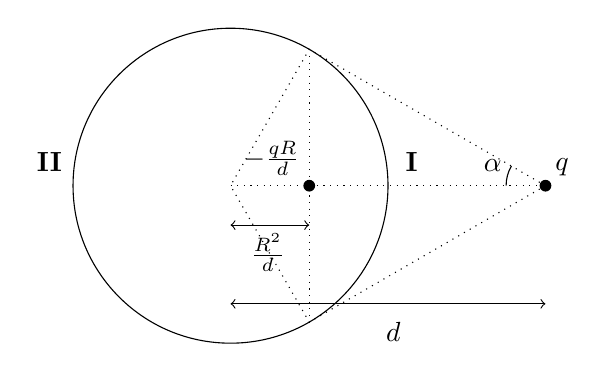
\begin{tikzpicture}
			\draw (0,0) circle (2);
			\draw[dotted] (0,0) -- (4,0);
			\draw[dotted] (4,0) -- (1,1.732) -- (0,0);
			\draw[dotted] (4,0) -- (1,-1.732) -- (0,0);
			\draw[dotted] (1,1.732) -- (1,-1.732);

			\node at (1,0)[circle,fill,inner sep=1.5pt]{};
			\draw (1,0) node[anchor=south east]{$-\frac{qR}{d}$};
			\draw (4,0) node[anchor=south west]{$q$};
			\node at (4,0)[circle,fill,inner sep=1.5pt]{};
			\draw[<->] (0,-0.5) -- (1, -0.5) node[xshift=-15,yshift=-10]{$\frac{R^2}{d}$};
			\draw[<->] (0,-1.5) -- (4, -1.5) node[xshift=-55,yshift=-10]{$d$};
			\draw (2.3,0.3) node{$\mathbf{I}$};
			\draw (-2.3,0.3) node{$\mathbf{II}$};
			\draw (3.5,0) arc (180:150:0.5) node[anchor=east]{$\alpha$};
		\end{tikzpicture}
	\end{center}
	We need the ratio of charge on $\mathbf{I}$ and $\mathbf{II}$
	\begin{equation}
		\frac{\iint_\mathbf{I}\sigma\,dS}{\iint_\mathbf{II}\sigma\,dS}
	\end{equation}
	But remember, $\sigma = \epsilon_0\vec{E}\hat{n}$, because this is a conductor. Replacing this in the above ratio, we get
	\begin{equation}
		= \frac{\iint_\mathbf{I}\vec{E}\cdot d\vec{S}}{\iint_\mathbf{II}\vec{E}\cdot d\vec{S}} = \frac{\text{Flux}_{\mathbf{I}}}{\text{Flux}_{\mathbf{II}}}
	\end{equation}
	Here we are talking about flux of the electric field. Now, as we can see contribution of $q$ towards flux through $I$ and $II$ is the same (except for the sign), and is $\frac{q\Omega}{4\pi\epsilon_0}$, where $\Omega$ is the solid angle subtended by the sphere on $q$. \\
	But $\Omega = 2\pi(1-\cos\alpha) = 2\pi\left(1-\frac{\sqrt{d^2-R^2}}{d}\right)$. So the flux due to $q$ is $\frac{q\left(1-\frac{\sqrt{d^2-R^2}}{d}\right)}{2\epsilon_0}$ through $\mathbf{II}$ and $-\frac{q\left(1-\frac{\sqrt{d^2-R^2}}{d}\right)}{2\epsilon_0}$ through $\mathbf{I}$\\
	Now, the flux due to the image charge $-\frac{qR}{d}$ is $-\frac{qR}{2\epsilon_0d}$ through both $\mathbf{I}$ and $\mathbf{II}$ \\
	So ultimately,
	\begin{equation}
		\frac{-\frac{q\left(1-\frac{\sqrt{d^2-R^2}}{d}\right)}{2\epsilon_0} -\frac{qR}{2\epsilon_0d} }{\frac{q\left(1-\frac{\sqrt{d^2-R^2}}{d}\right)}{2\epsilon_0} - \frac{qR}{2\epsilon_0d}} = \frac{R + d - \sqrt{d^2-R^2}}{R - d + \sqrt{d^2 - R^2}} = \sqrt{\frac{d+R}{d-R}} \hskip0.3\textwidth\blacksquare
	\end{equation}
\end{solution}

\question Two infinite conducting plates (both grounded and perpendicular to the $x-y$ plane) meet at an angle of $60 \degree$. A point charge $+q$ in the $xy$ plane has plane polar coordinates $(a, 20 \degree)$. Find all the image charges and their positions in polar coordinates.
\begin{solution}
	\begin{center}
			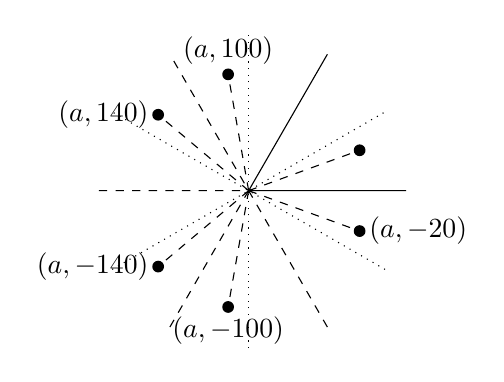
\begin{tikzpicture}

				\draw (1, 1.732) -- (0,0) -- (2,0);
				\draw[dotted] (-1.732,-1) -- (1.732,1);
				\draw[dotted] (1.732,-1) -- (-1.732,1);
				\draw[dotted] (0,-2) -- (0,2);

				\draw[dashed] (0,0) -- ({1.5 * cos(20)},{1.5 * sin(20)});
				\draw[dashed] (0,0) -- ({1.5 * cos(20)},-{1.5 * sin(20)}) node[anchor=west]{$(a,-20\degree)$};
				\draw[dashed] (0,0) -- (-{1.5 * sin(10)},{1.5 * cos(10)}) node[anchor=south]{$(a,100\degree)$};
				\draw[dashed] (0,0) -- (-{1.5 * sin(10)},-{1.5 * cos(10)}) node[anchor=north]{$(a, -100\degree$)};
				\draw[dashed] (0,0) -- (-{1.5 * cos(40)},{1.5 * sin(40)}) node[anchor=east]{$(a, 140\degree)$};
				\draw[dashed] (0,0) -- (-{1.5 * cos(40)},-{1.5 * sin(40)}) node[anchor=east]{$(a, -140\degree)$};

				\node at ({1.5 * cos(20)},{1.5 * sin(20)})[circle,fill,inner sep=1.5pt]{};
				\node at ({1.5 * cos(20)},-{1.5 * sin(20)})[circle,fill,inner sep=1.5pt]{};
				\node at (-{1.5 * sin(10)},{1.5 * cos(10)})[circle,fill,inner sep=1.5pt]{};
				\node at (-{1.5 * sin(10)},-{1.5 * cos(10)})[circle,fill,inner sep=1.5pt]{};
				\node at (-{1.5 * cos(40)},{1.5 * sin(40)})[circle,fill,inner sep=1.5pt]{};
				\node at (-{1.5 * cos(40)},-{1.5 * sin(40)})[circle,fill,inner sep=1.5pt]{};

				\draw[dashed] (1,-1.732) -- (-1, 1.732);
				\draw[dashed] (-1, -1.732) -- (0,0) -- (-2,0);
			\end{tikzpicture}
		\end{center}
\end{solution}

\question A rectangular pipe running parallel to the $z$-axis (from $-\infty$ to $+\infty$) has three grounded metal sides at $y = 0, y = a$ and $x = 0$. The fourth side at $x = b$ is maintained at a specified potential $V_0(y)$.
\begin{parts}
	\part Develop a general formula for the potential within the pipe.
	\begin{solution}
		We need to solve 
	$$
	\frac{\partial^2V}{\partial x^2}+\frac{\partial^2V}{\partial y^2}= 0
	$$
	with the boundary conditions given as 
	\begin{equation*}
	\begin{split}
	&V(x,0)=0\\
	&V(x,a)=0\\
	&V(0,y)=0\\
	&V(b,y)=V_0(y)
	\end{split}  
	\end{equation*}
	Using separation of variables, the solution to the above equation can be written as 
	$$
	V(x,y) = \left(Ae^{kx}+Be^{-kx}\right)\left(C\sin ky + D\cos ky\right)
	$$
	Using the boundary conditions we can deduce that 
	\begin{equation*}
	\begin{split}
	&D=0\\
	&B=-A\\
	&k=\frac{n\pi}{a}\\
	\end{split}
	\end{equation*}
	Using the above we can write the most general form of the solution as 
	$$
	V(x,y) = \sum_{n=1}^{\infty}C_n\sinh(n\pi x/a)\sin(n\pi y/a)
	$$
	wherein $C_n$ can be determined using the boundary condition $V(b,y)=V_0(y)$ and is given as 
	$$
	C_n = \frac{2}{a \sinh(n\pi b/a)}\int_0^a V_0(y)\sin(n\pi y/a)dy
	$$
	\end{solution}

	\part Find the potential explicitly, for the case $V_0(y) = V_0$ (a constant).
	\begin{solution}
		In this case $C_n$ turns out to be 
		\begin{equation*}
		C_n = \frac{2}{a \sinh(n\pi b/a)} V_0\int_0^a \sin(n\pi y/a)dy\\
		\end{equation*}
		The integral in the above eq. is 0 when $n$ is even and $\frac{2a}{n\pi}$ when $n$ is odd. So, finally we will get 
		$$
		V(x,y) = \frac{4V_0}{\pi}\sum_{n=1,3,5}\frac{\sinh(n\pi x/a)\sin(n\pi y/a)}{n \sinh(n\pi b/a)}
		$$

	\end{solution}
\end{parts}

\end{questions}
\end{document}